\documentclass[conference]{IEEEtran}
\IEEEoverridecommandlockouts
% The preceding line is only needed to identify funding in the first footnote. If that is unneeded, please comment it out.
\usepackage[brazilian]{babel}
\usepackage{cite}
\usepackage{amsmath,amssymb,amsfonts}
\usepackage{algorithmic}
\usepackage{graphicx}
\usepackage{textcomp}
\usepackage{xcolor}
\usepackage[show]{ed}
\usepackage{tabularx}

\def\BibTeX{{\rm B\kern-.05em{\sc i\kern-.025em b}\kern-.08em
    T\kern-.1667em\lower.7ex\hbox{E}\kern-.125emX}}

%comandos para o meu comentário
\newcommand{\xexeo}[1]{\ednote{\textcolor{red}{Xexéo - #1}}}
\newcommand{\carla}[1]{\ednote{\textcolor{purple}{Carla - #1}}}
\newcommand{\julio}[1]{\ednote{\textcolor{blue}{Júlio - #1}}}
\newcommand{\horacio}[1]{\ednote{\textcolor{navy}{Horácio - #1}}}
    
\newcolumntype{Y}{>{\centering\arraybackslash}X}
    
\begin{document}

\title{Léo \& Maya: um jogo para auxiliar no ensino de pensamento computacional paralelo
}

%\author{
\IEEEauthorblockN{[AVALIAÇÃO CEGA]}
\IEEEauthorblockA{[AVALIAÇÃO CEGA]}
}

\author{
\IEEEauthorblockN{Horácio B. M. Henriques}
\IEEEauthorblockA{\textit{Instituto de Computação} \\\textit{Universidade Federal do Rio de Janeiro}\\Rio de Janeiro, Brasil \\horacio97@dcc.ufrj.br}\\
\IEEEauthorblockN{Carla A. D. M. Delgado}
\IEEEauthorblockA{\textit{Instituto de Computação} \\\textit{Universidade Federal do Rio de Janeiro} \\Rio de Janeiro, Brasil \\carla@dcc.ufrj.br}\\
\and
\IEEEauthorblockN{Júlio R. K. Mandoju}
\IEEEauthorblockA{\textit{Instituto de Computação} \\\textit{Universidade Federal do Rio de Janeiro} \\Rio de Janeiro, Brasil \\juliorkm@dcc.ufrj.br} \\
\IEEEauthorblockN{Geraldo Xexéo}
\IEEEauthorblockA{\textit{Prog. de Engenharia e Sistemas de Informação} \\\textit{COPPE}\\\textit{Instituto de Computação}\\\textit{Universidade Federal do Rio de Janeiro}\\Rio de Janeiro, Brasil \\gxexeo@cos.ufrj.br}
}

\maketitle


\begin{abstract}
Em um mundo com cada vez mais computadores, é imprescindível que as pessoas saibam resolver problemas usando computadores de forma eficaz. Para tal, é necessário introduzir pessoas ao Pensamento Computacional: um meio de resolver problemas que consiste em interpretar e dividir problemas grandes em problemas menores com soluções conhecidas e descrever essa solução na forma de um algoritmo. O jogo Léo \& Maya é uma forma de ajudar no ensino de Pensamento Computacional para crianças de sete a onze anos. Ele consiste em vinte e duas fases de complexidade crescente onde o jogador é levado a montar algoritmos usando um conjunto específico de instruções para completar objetivos específicos, por vezes fazendo uso de Pensamento Computacional Paralelo para controlar mais de um personagem dentro de uma fase. Apesar da validação ter ocorrido durante a pandemia do Covid-19, que limitou o acesso aos voluntários entrevistados, a recepção por parte dos professores entrevistados, responsáveis por alunos dentro da faixa etária pretendida foi positiva, apontando para um futuro promissor para o projeto.
\end{abstract}

\renewcommand{\IEEEkeywordsname}{Palavras-Chave}
\begin{IEEEkeywords}
Pensamento Computacional, Pensamento Computacional Paralelo, Jogos Educativos.
\end{IEEEkeywords}

\section{Introdução}

Pensamento Computacional (PC) é um assunto que tem ganhado cada vez mais relevância ao longo dos últimos anos em discussões sobre educação infantil \cite{barr_bringing_2011}. Citado pela primeira vez por Jeanette Wing em 2006, PC foi vagamente definido como ``resolução de problemas, idealização de sistemas e compreensão do comportamento humano através de conceitos fundamentais à Ciência da Computação''\cite{wing_computational_2006} e, desde então, se constitui em objeto de discussão no meio acadêmico, da definição até a aplicabilidade em salas de aula.

Hoje em dia, compreende-se que PC seja um conjunto de habilidades necessárias, comumente divididas em quatro pilares: abstração, decomposição em subproblemas, reconhecimento de padrões e criação de algoritmos\cite{brackmann_desenvolvimento_2017}. Essas habilidades seriam úteis não só para um programador que precisa escrever códigos com algum objetivo prático, mas para qualquer pessoa que precise resolver um problema.

Cada vez mais currículos de ensino médio e ensino fundamental estão agregando conteúdos de PC. Por exemplo, o plano de currículo K-12, dos Estados Unidos tem ``flertado'' com conceitos de PC desde 2011\cite{barr_bringing_2011}, vindo a cada vez mais empregar esforços ao longo de anos para agregar conteúdos de PC no currículo de crianças e adolescentes. Já no Brasil, a Base Nacional Comum Curricular (BNCC) aprovada em dezembro de 2017 menciona explicitamente, na seção de Ensino Matemático, aplicações de álgebra no desenvolvimento de PC através do uso de algoritmos como estratégia para resolver problemas matemáticos\cite{ministerio_da_educacao_base_2018}.

Currículos escolares normalmente não abordam o assunto de Pensamento Computacional Paralelo (PC-Paralelo). Por mais que tenha sido mencionado por Wing em 2006 em seu primeiro artigo seminal sobre o assunto, e mais uma vez investigado em maior detalhe por Kirkpatrick no artigo "Parallel Computer Thinking" em 2017, PC-Paralelo é tido como um assunto que pode ser complexo demais para um aluno ter tempo de aprender em sala de aula, apesar de sua importância\cite{kirkpatrick_parallel_2017}.

De modo a auxiliar o ensino de PC para jogadores em idade escolar e tentar cobrir essa lacuna,  foi desenvolvido o jogo educativo endógeno Léo \& Maya.  O objetivo é ensinar, através de uma abordagem lúdica, como fazer uso de PC para a resolução de problemas que admitem soluções algorítmicas, contemplando também o ensino de PC-Paralelo. Os ensinamentos serão passados através de várias fases onde os jogadores montarão algoritmos que serão seguidos pelos personagens do jogo — o gato Léo e a cachorra Maya — de modo a solucionar o problema proposto pela fase.

\section{Fundamentação Teórica}

\subsection{Pensamento Computacional e Pensamento Computacional Paralelo}

PC envolve resolver subproblemas, desenhar sistemas e compreender comportamento humano ao se utilizar de conceitos fundamentais à Ciência da Computação\cite{wing_computational_2006}. É uma forma de pensamento e resolução de problemas que influencia outros campos de estudo fora da computação, como ``Medicina Algorítmica, Arqueologia Computacional, Economia Computacional, Finanças Computacionais, Computação e Jornalismo, Direito Computacional, Ciências Sociais Computacionais e Humanidades Digitais''\cite{wing_computational_2010}. E mesmo fora destes campos de estudo, PC é útil uma vez que dá às pessoas a capacidade de adaptar soluções algorítmicas, avaliar quando um computador é melhor indicado para lidar com um problema e aplicar estratégias como divisão e conquista na resolução de problemas na vida cotidiana\cite{wing_computational_2010}.

PC é uma habilidade comumente relacionada com currículos de Computação\cite{tch060} ou Matemática, uma vez que os alunos precisam ``ser capazes de traduzir uma situação dada em outras linguagens, como transformar situações-problema, apresentadas em língua materna, em fórmulas, tabelas e gráficos, e vice-versa''\cite{ministerio_da_educacao_base_2018} para a aprendizagem de Álgebra e outros campos da Matemática. 

A discussão sobre o ensino de PC não é atual, tendo em vista que ações para o Ensino de Computação a crianças, como, por exemplo, o uso de LOGO ou de Basic para fins didáticos, são discutidas desde os anos 80\cite{grover_computational_2013}. A discussão foi renovada quando, em 2006, Wing definiu em seu artigo ``Computational Thinking'' o que é PC, e estabeleceu a importância dessa prática. Desde então, trabalhos têm sido produzidos de modo a explorar formas de integrar o ensino de PC em turmas de ensino fundamental e médio\cite{wing_computational_2006}\cite{de_franca_disseminacao_2014}\cite{repenning_computational_2016}\cite{monclar_jogos_nodate}.

Contudo, já em 2021, as pessoas têm amplo acesso a computadores, \textit{smartphones} e \textit{tablets} com multiprocessadores, que permitem a todo tipo de aplicação executar tarefas em paralelo, algo que não era comum até aproximadamente uma década atrás, quando a Computação Paralela se tornou convencional. Portanto, é importante que se contemple também o ensino de PC-Paralelo, que traz consigo muitas vantagens\cite{BBC}.

Um dos benefícios da Computação Paralela é ajudar ``a desenvolver uma abordagem mais flexível para solucionar problemas, porque há mais modelos nos quais se basear.''\cite{BBC} Além disso, o paralelismo oferece mais formas de quebrar um problema grande em subproblemas menores, algo que pode acrescentar às vantagens de se aprender o PC, considerando que a decomposição de problemas é um de seus pilares fundamentais\cite{BBC}.

\subsection{Jogos Educativos Endógenos}
  
%definição de jogo do Jesper Juul + crianças se interessam por conhecimentos que lhe façam sentido de acordo com Piaget
A definição de jogo é tema de discussão há décadas, sendo assim impossível declarar uma definição como definitiva. Por esse motivo, a definição adotada neste trabalho é a definição encontrada no livro \textit{Half-Real: Video Games between Real Rules and Fictional Worlds}, onde jogos são definidos em uma lista de seis tópicos que tem como sexto tópico "as consequências da atividade (de jogar) são opcionais e negociáveis"\cite{halfreal}. Esta definição nos é cômoda uma vez que admite que o ato de jogar pode ter consequências na vida real (no emprego do termo "negociável") para além de uma atividade lúdica ou social, podendo desta forma servir para educar o jogador sobre algum assunto. Esta definição também nos permite fazer uma ponte com a teoria construtivista de Jean Piaget, que defendia que o conhecimento se constrói através da exploração do objeto de estudo, e não de uma transmissão unilateral de conhecimento entre aluno e professor\cite{novaescola_piaget}. %Esta teoria pode ser vista refletida nos trabalhos de Seymour Papert e Paulo Freire, que visavam colocar o aluno como protagonista do próprio aprendizado\cite{soffner}.
  
Quando se discutem jogos educativos, é importante levar em conta como o conteúdo pedagógico a ser ensinado para o jogador está integrado no jogo, uma vez que o sucesso do jogo como atividade didática depende do quão intrínsecos são os conteúdos abordados dentro da fantasia oferecida pelo jogo \cite{habgood_endogenous_2005}. Nisso, podemos aqui ver a divisão de jogos educativos em duas categorias: os jogos educativos sendo exógenos ou endógenos\cite{halverson_what_nodate}.

O jogo educativo exógeno é, por natureza, mais fácil de ser feito e executado, por isso tem tido maior adoção por professores.\cite{halverson_what_nodate} A característica mais marcante desse tipo de jogo educativo é a ausência de ligação entre as regras e o conteúdo que se quer ensinar.  Um exemplo desse tipo de jogo seriam perguntas-e-respostas, onde as regras do jogo independem do conteúdo das perguntas e meramente coexistem com o conteúdo.

Por outro lado, o jogo educativo endógeno possui necessariamente uma ligação entre o \textit{game design} e o conteúdo a ser passado. Sua maior característica é fazer com que o domínio do jogo venha agregado ao domínio do próprio conteúdo. Exemplos conhecidos são os jogos de estratégia históricos, como as séries Civilization e Rise of Nations\cite{halverson_what_nodate}.

Jogos educativos endógenos são presentes em lojas virtuais de jogos eletrônicos, abordando vários temas. Um desses temas é a programação de soluções na forma de algoritmos em ambientes simulados\cite{googleplay}\cite{gogcom}\cite{steam_tag_programming}. A existência de outros jogos que abordam conteúdos similares a Léo \& Maya é excelente, uma vez que prova a existência de um mercado para esse tipo de jogo e informa uma coleção de convenções e ideias sobre as quais o nosso jogo pode construir.

Léo \& Maya tira grande inspiração de Human Resource Machine\cite{humanresourcemachine}, uma vez que ambos são jogos que podem ser jogados em celulares e computadores, e se baseiam em fazer o jogador programar algoritmos para resolver problemas  divididos em fases. Contudo, Léo \& Maya se diferencia da maioria abordando paralelismo desde as primeiras fases e algoritmos através de uma sintaxe simplificada.

\section{Projeto do Jogo Educativo}

Antes do desenvolvimento do jogo, criou-se um \textit{game design canvas} baseado no Game Design Canvas para jogos endógenos (Endo-GDC) de modo a ``facilitar a discussão e descrição de um jogo sério''\cite{taucei_endo-gdc_nodate}. O canvas é útil para unificar a linguagem usada por todas as partes envolvidas na produção do \textit{game} e descrever de forma explícita e legível a relação entre o conteúdo que se quer passar, os objetivos pedagógicos que querem ser atingidos através do conteúdo e as mecânicas do jogo que deverão ter ligação direta com os objetivos. Todo o conteúdo desse canvas foi, num momento posterior, traduzido em um documento de \textit{game design}. 

%Como o GDC foi usado: alunos de CC com experiência prévia em desenvolvimento de jogo
O Endo-GDC foi usado neste trabalho por dois alunos de bacharelado de Ciência da Computação com experiência na produção de jogos eletrônicos. Os alunos contaram com a orientação de professores orientadores interessados no campo da educação e sua relação com computação no momento de adquirir os conhecimentos necessários para definir os campos do canvas fora da área de domínio. Para tal, os alunos e orientadores conduziram discussões sobre currículos escolares atuais, o mercado de jogos educativos com foco em ensino de PC e tópicos menos abordados por esses jogos comerciais. A partir destas discussões, houve o estudo de currículos para definir conteúdos \cite{govuk} \cite{tch060}, o uso da Taxonomia Revisada de Bloom para definir objetivos pedagógicos \cite{krathwohl} e um estudo de jogos similares como forma de identificar mecânicas que possam ser familiares para jogadores.

\def\tabularycolumn#1{m{#1}}
\begin{table}[htbp]
\caption{Relação entre objetivos de aprendizado e mecânicas do jogo ``Léo \& Maya''}
\begin{center}
\begin{tabularx}{9cm}{|Y|Y|Y|Y|Y|}
\hline
\textbf{ }&\textbf{Reconhecer\linebreak subproble-\linebreak mas}&\textbf{Interpretar\linebreak objetivo}&\textbf{Analisar\linebreak limitações}&\textbf{Conceber\linebreak algoritmos} \\
\hline
\textbf{Trilha de instruções de tamanho finito} & & & & X  \\
\hline
\textbf{Andar pelo mapa} & & X & X & X \\
\hline
\textbf{Empurrar objetos} & & & X & X\\
\hline
\textbf{Pegar ou largar objetos} & & X & X & X\\
\hline
\textbf{Árvores} & & & X & X\\
\hline
\textbf{Laços de instruções} & X & & X & X\\
\hline
\textbf{Dois personagens jogáveis} & X & X & X & X\\
\hline
\textbf{Barreiras} & X & & X & X\\
\hline
\end{tabularx}
\label{tab1}
\end{center}
\end{table}

A relação entre objetivos pedagógicos e mecânicas é resumida na tabela 1, onde cada linha da tabela corresponde a uma mecânica do jogo e cada coluna corresponde a um objetivo pedagógico. Cada célula da tabela marcada com um ``X'' representa a relação entre uma mecânica e um objetivo pedagógico específicos, podendo assim uma mecânica ter relação com mais de um objetivo pedagógico ao mesmo tempo.

O conteúdo pedagógico que o jogo aborda está alinhado com currículos de cursos de programação ao redor do mundo\cite{tch060}\cite{govuk}, introduzindo conteúdos pontuais desses mesmos currículos na ordem em que eles aparecem nos planos de aulas. A diferença é a introdução de paralelismo por parte do jogo, conteúdo que não aparece em nenhum dos currículos consultados. Através dos conteúdos pedagógicos, o jogo visa exercitar a construção de algoritmos e a divisão de problemas complexos em subproblemas simples de solução conhecida, dois dos quatro pilares fundamentais de PC\cite{BBC}.

No que diz respeito aos aspectos técnicos, utilizou-se a \textit{Unity}\cite{unity} para construir o jogo. A \textit{Unity} é um motor de jogos gratuito estabelecido no mercado que permite a criação de aplicações com recursos gráficos tanto em 2D quanto 3D, e que possui um foco no mercado de desenvolvimento de jogos eletrônicos. Atualmente, a Unity utiliza C\#\cite{wagner_documentacao_nodate} como a linguagem para escrever \textit{scripts} dentro dos projetos, e permite a exportação dos seus projetos para, dentre outras plataformas, computadores pessoais e celulares \textit{Android}. Além disso, toda a arte do jogo foi produzida usando o aplicativo pago \textit{Aseprite}\cite{aseprite}.

O jogo possui um total de vinte e duas fases divididas em seis seções que introduzem mecânicas e conteúdos diferentes. As fases do jogo funcionam todas praticamente da mesma forma, de modo a manter a consistência na interação do jogador com as mecânicas do jogo e não exigir que o jogador reaprenda a jogar a cada fase. Caso a fase seja a primeira de alguma seção e o jogador estiver jogando a fase pela primeira vez, um vídeo demonstra através de um exemplo a mecânica nova que o conjunto de fases introduz.

Ao abrir uma fase, o jogador tem acesso à visão inteira do mapa da fase, a uma descrição do objetivo e não tem restrição de tempo para conceber uma resposta. Desde o início da fase, o jogador é livre para arrastar instruções, representadas por artefatos visuais, até a trilha de instruções localizada no canto da tela.

\begin{figure}[htbp]
\centerline{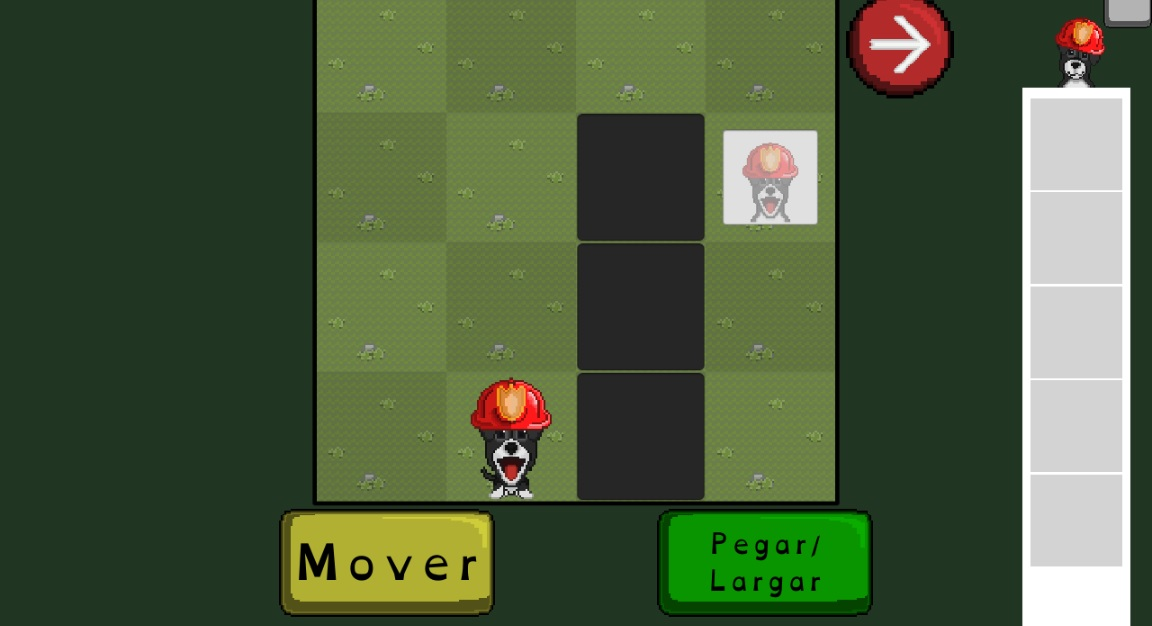
\includegraphics[scale=0.275]{images/fig01.jpg}}
\caption{Início da fase 5-1, a primeira fase que aborda laços de instruções.}
\label{fig}
\end{figure}

Assim que o jogador se der por satisfeito com a solução concebida, ele deve apertar no botão ``pronto'' para dar continuidade. Se o jogo não tiver introduzido laços de instruções, o jogador será levado diretamente para a execução do algoritmo. Caso contrário, o jogador terá a liberdade de definir laços de instruções com um número finito de repetições em uma segunda tela. Nesta tela, o jogador também tem a liberdade de retornar para a anterior e fazer algum ajuste às instruções presentes na trilha.

Uma vez que o algoritmo seja iniciado, o jogo o executará até que um dos dois cenários ocorram: ou os personagens da fase cumprem os objetivos propostos pela fase, ou não. Em caso de sucesso, o jogador terá a opção de voltar ao menu principal e seguir para a próxima fase ou jogar a mesma fase novamente. Caso contrário, o jogo explicará o que aconteceu de errado na execução do algoritmo e permitirá que o jogador jogue a fase de novo, preservando a solução errada para correção.

\section{Validação}

A validação do trabalho se deu durante a pandemia do Covid-19, o que foi um desafio por si só. Além da pandemia, o público-alvo do jogo são menores de idade, o que motivou a fazer a validação com professores de diferentes faixas etárias, de modo a contemplar também a impressão que o jogo pode causar em pessoas de fora da faixa etária pretendida. Desta forma, a validação se deu na forma de uma pesquisa qualitativa onde, através de mensagens eletrônicas por \textit{e-mail} e \textit{facebook}, professores receberam o link para acessar o jogo, um questionário com uma explicação breve sobre PC e cinco páginas com perguntas sobre o histórico do professor acerca do uso de jogos didáticos e a opinião sobre diferentes aspectos do jogo. As respostas do formulário foram armazenadas em uma planilha para análise.

Durante a busca por professores voluntários, de modo a contemplar pontos de vista de pessoas de fora da área e fazer Léo \& Maya ser mais acessível para indivíduos sem conhecimento prévio sobre PC, professores de todas as matérias foram entrevistados. Ao final da pesquisa, onze voluntários responderam ao formulário. Destes onze, três deles dão aula para a faixa etária alvo do jogo, enquanto que os outros oito dão aula para alunos mais velhos ou mais novos; e sete deles dão aula de Matemática e/ou Computação. Um dos professores entrevistados leciona especificamente a matéria "Pensamento Computacional" para alunos de cinco a sete anos.

As respostas mostraram que, na opinião do público entrevistado, o jogo Léo \& Maya é apropriado tanto como atividade didática quanto lúdica, para crianças em idades entre cinco e catorze anos, o que é mais amplo do que a faixa etária pretendida. Professores voluntários com alunos na faixa etária de quinze a dezessete anos, contudo, se dividem sobre a adequação do jogo para seus alunos. Para professores com alunos em faixas etárias abaixo dos cinco anos ou acima dos dezoito anos, o jogo se mostrou inadequado, como esperado.

Em sua maioria, os professores voluntários indicaram que o jogo também ajuda no ensino de dois pilares específicos de PC: a abstração e concepção de algoritmos. Apesar de os voluntários não serem familiarizados com o conceito de PC, essa opinião foi corroborada pelo único professor que leciona a matéria.

A recepção por parte dos voluntários foi positiva, uma vez que nenhum professor voluntário reportou ter desgostado do jogo por completo. O questionamento mais comum entre os professores foi sobre os tutoriais, que precisam ser repensados para ensinar melhor a jogar. Além disso, foi citada a falta de \textit{feedback} audiovisual em tempo real ao bater em paredes, o que torna a mensagem de erro que aparece confusa.

\section{Conclusão e Trabalhos Futuros}

PC é uma habilidade cada vez mais relevante tanto em currículos escolares quanto na vida cotidiana. E recentemente, com a inclusão de PC em currículos escolares, que costumam relacionar esse conteúdo com matérias dedicadas à Computação ou álgebra, a discussão sobre como exercitar tal habilidade tem tomado maior relevância. Com o objetivo de ajudar no ensino de PC, criou-se Léo \& Maya: um jogo educativo para computadores pessoais e celulares \textit{Android} feito em \textit{Unity} voltado para o público em idade escolar sobre uma cachorra e um gato bombeiros que ajudam animaizinhos em apuros que visa ensinar sobre PC sequencial e paralelo. Ao longo de vinte e duas fases, o jogo busca ensinar sobre construção de algoritmos para resolver problemas e reconhecimento de subproblemas dentro de problemas grandes, ao mesmo tempo em que familiariza seu público com o conceito de paralelizar soluções de problemas e lidar com as condições em que isso implica. 

Para o futuro próximo, existe o objetivo de retrabalhar os tutoriais de modo que eles sejam mais acessíveis a um número maior de pessoas na hora de ensinar como jogar o jogo. Também existe a ambição de colocar artifícios de comunidade, como uma forma de criar fases customizáveis e de compartilhar estas mesmas fases e \textit{leaderboards} para estimular competitividade entre jogadores e aperfeiçoamento na hora de montar algoritmos, e implementar uma quantidade maior de arte de modo a fazer o jogo mais sensorialmente agradável de se jogar.

\bibliography{biblio.bib}
\bibliographystyle{IEEEtran}

\end{document}
